% coding: utf-8
% --------------------------------------------------------------------------------------------------
% "Синтез оптимального стохастического управления", 2011 год
% --------------------------------------------------------------------------------------------------



\documentclass[ignorenonframetext,hyperref={pdftex,unicode},compress]{beamer}
\mode<presentation>{}

\usepackage{cmap}
\usepackage[utf8x]{inputenc}
\usepackage[russian]{babel}
\usepackage[T2A]{fontenc}
\DeclareSymbolFont{T2Aletters}{T2A}{cmr}{m}{it}
\selectlanguage{russian}

\PrerenderUnicode{О проблемах синтеза оптимального регулятора с обратной связью в многомерных стохастических системах}

\hypersetup{
    pdftitle={О проблемах синтеза оптимального регулятора с обратной связью в многомерных стохастических системах},
    pdfauthor={Сергей Архипов},
    pdfsubject={Магистерская диссертация},
    pdfkeywords={Оптимальное управление} {Стохастические системы} {Полет ракеты}
}

\usepackage{amssymb}
\usepackage{amsfonts}
\usepackage{amsmath}
\usepackage{mathtext}
\usepackage[mathscr]{eucal}
\usepackage[russian]{varioref}
\usepackage{listings}
\usepackage[font=it,labelsep=period,format=hang]{caption}



\usepackage{microtype}
\SetProtrusion
{
encoding = T2A,
family = cmr
}
{
« =  {1000,     },
» =  {    , 1000},
„ =  {1000,     },
“ =  {    , 1000},
( =  {1000,     },
) =  {    , 1000},
! =  {    , 1000},
? =  {    , 1000},
: =  {    , 1000},
; =  {    , 1000},
. =  {    , 1000},
- =  {    , 1000},
{,}= {    , 1000}
}
\DeclareMicrotypeSet{t2atext}{encoding=T2A}
\UseMicrotypeSet{t2atext}



% for screen only
\usetheme{Singapore}

% for handout only
%\usetheme{Pittsburgh}
%\usecolortheme{dove}


\newcommand{\br}{\vspace{12pt}}
\newtheorem{teo}{Теорема}
\newtheorem{alg}{Алгоритм}



%-------------------------------------------------------------------------------



\title{О проблемах синтеза оптимального регулятора с обратной связью в многомерных стохастических системах}
\author{Архипов С.\,В.}
\institute{Научный руководитель: Пакшин П.\,В.}
\date{15 июня 2011 г.}



\begin{document}



%-------------------------------------------------------------------------------
%---   слайд 0: титульная страница
%-------------------------------------------------------------------------------
\begin{frame}
    \titlepage
\end{frame}



%-------------------------------------------------------------------------------
%---   слайд 1: постановка основной задачи
%-------------------------------------------------------------------------------
\begin{frame}
	\frametitle{Постановка задачи}

    Пусть физический объект описывается системой

	\begin{equation}\label{eq:1}
	    \dot{\mathbf{x}}(t) = \mathbf{A}(t)\mathbf{x}(t) + \mathbf{B}(t)\mathbf{u}(t) \text{.}
	\end{equation}

	Требуется найти такое оптимальное управление $\mathbf{u}^*(t)$, при котором значение критерия качества было бы минимальным:
	
	\begin{equation}\label{eq:2}
	    \mathcal{F} \bigl(  \mathbf{x}(t), \mathbf{u}^*(t)  \bigr) = \min_{\mathbf{u}(t) \in \Upsilon} \mathcal{F} \bigl(  \mathbf{x}(t), \mathbf{u}(t)  \bigr)  \text{.}
	\end{equation}
\end{frame}



%-------------------------------------------------------------------------------
%---   слайд 2: Синтез оптимального управления -- уравнение Беллмана
%-------------------------------------------------------------------------------
\begin{frame}
	\frametitle{Синтез оптимального управления}
	\framesubtitle{Уравнение Беллмана}

    Пусть критерий качества задан в виде
    
    \begin{equation}\label{eq:3}
    	\mathcal{F} = \int\limits_{t_1}^{t_2} \mathsf{L}(\mathbf{x}, \mathbf{u}, t)\,dt \text{.}
    \end{equation}
    
    Тогда необходимое условие оптимальности запишется как
    
    \begin{equation}\label{eq:4}
    	\underset{\mathbf{u}(t) \in \Upsilon}{\min} \biggl\{ \biggl[ \frac{d \mathcal{F}^*}{d t} \biggr]_{\mathbf{u}, t} + \mathsf{L}\bigl(  \mathbf{x}(\mathbf{u}, t), \mathbf{u}, t  \bigr) \biggr\} = 0 \text{.}
    \end{equation}
\end{frame}



%-------------------------------------------------------------------------------
%---   слайд 3: Синтез оптимального управления -- уравнение Беллмана, квадратич-
%---            ный критерий качества
%-------------------------------------------------------------------------------
\begin{frame}
	\frametitle{Синтез оптимального управления}
	\framesubtitle{Уравнение Беллмана с квадратичным критерием качества}\small

    Пусть критерий качества задан в виде
    
    \begin{equation}\label{eq:5}
    	\mathcal{F} = \frac{1}{2} \mathbf{x}_2^T \mathbf{M} \mathbf{x}_2 + \frac{1}{2} \int\limits_{t_1}^{t_2} \bigl[ \mathbf{x}^T(\tau)\mathbf{Q}(\tau)\mathbf{x}(\tau) + \mathbf{u}^T(\tau)\mathbf{R}(\tau)\mathbf{u}(\tau) \bigr]\,d\tau \text{.}
    \end{equation}
    
    Тогда оптимальное управление $\mathbf{u}^*(t)$ может быть синтезировано следующим образом:
    
    \begin{equation}\label{eq:6}
    	\mathbf{u}^*(\mathbf{x}, t) = -\mathbf{R}^{-1}(t)\mathbf{B}^T(t)\mathbf{P}(t)\mathbf{x}(t) \text{,}
    \end{equation}
    
    где матрица $\mathbf{P}(t)$ может быть найдена из уравнения Риккати
    
    \begin{equation}\label{eq:7}
    	\begin{cases}
    		\begin{split}
    			- \frac{d \mathbf{P}(t)}{dt} =& -\mathbf{P}(t)\mathbf{B}(t)\mathbf{R}^{-1}(t)\mathbf{B}^T(t)\mathbf{P}(t) + \mathbf{P}(t)\mathbf{A}(t) + \\
    			&+ \mathbf{A}^T(t)\mathbf{P}(t) + \mathbf{Q}(t) \text{;}
			\end{split} \\
			\mathbf{P}(t_2) = \mathbf{M} \text{.}
		\end{cases}    
    \end{equation}
\end{frame}



%-------------------------------------------------------------------------------
%---   слайд 4: Синтез оптимального управления -- уравнение Беллмана, стационар-
%---            ный случай
%-------------------------------------------------------------------------------
\begin{frame}
	\frametitle{Синтез оптимального управления}
	\framesubtitle{Уравнение Беллмана при $T \to \infty$}

    Пусть критерий качества задан в виде
    
    \begin{equation}\label{eq:8}
    	\mathcal{F} = \frac{1}{2} \int\limits_0^\infty \bigl[ \mathbf{x}^T(\tau)\mathbf{Q} \mathbf{x}(\tau) + \mathbf{u}^T(t)\mathbf{R} \mathbf{u}(\tau) \bigr]\,d\tau \text{.}
    \end{equation}
    
    Тогда оптимальное управление $\mathbf{u}^*(t)$ может быть синтезировано следующим образом:
    
    \begin{equation}\label{eq:9}
    	\mathbf{u}^*(\mathbf{x}, t) = -\mathbf{R}^{-1}\mathbf{B}^T\mathbf{P}\mathbf{x}(t) \text{,}
    \end{equation}
    
    где матрица $\mathbf{P}$ может быть найдена из нелинейного алгебраического матричного уравнения Риккати
    
    \begin{equation}\label{eq:10}
    	-\mathbf{P}\mathbf{B}\mathbf{R}^{-1}\mathbf{B}^T\mathbf{P} + \mathbf{P}\mathbf{A} + \mathbf{A}^T\mathbf{P} + \mathbf{Q} = \mathbf{0} \text{.}    
    \end{equation}
\end{frame}



%-------------------------------------------------------------------------------
%---   слайд 5: Оптимальное стохастическое управление - постановка задачи
%-------------------------------------------------------------------------------
\begin{frame}
	\frametitle{Оптимальное стохастическое управление}
	\framesubtitle{Постановка задачи}
    
    Пусть система задана в виде процесса Ито:

    \begin{equation}\label{eq:11}
    	d\mathbf{x}_t = \bigl( \mathbf{A}(t)\mathbf{x}_t + \mathbf{B}(t)\mathbf{u}(\mathbf{x}_t, t) \bigr)dt + \mathbf{C}(t)d\mathbf{w}_t \text{.}
    \end{equation}
    
    Тогда оптимальное управление $\mathbf{u}^*(t)$ синтезируется из условия минимума функционала качества:
    
    \begin{equation}\label{eq:12}
    	\mathcal{F}(\mathbf{x}, \mathbf{u}, s) = \mathbb{E} \biggl\{ Q(\mathbf{x}_\tau, \tau) + \int\limits_s^\tau F(\mathbf{x}_t, \mathbf{u}, t)\,dt~\biggm|~ \mathbf{x}_s = \mathbf{x} \biggr\} \text{.}
    \end{equation}
\end{frame}



%-------------------------------------------------------------------------------
%---   слайд 6: Оптимальное стохастическое управление - квадратичный критерий
%---            качества
%-------------------------------------------------------------------------------
\begin{frame}
	\frametitle{Оптимальное стохастическое управление}
	\framesubtitle{Синтез оптимального управления}\small
    
    Пусть критерий качества является квадратичным

    \begin{equation}\label{eq:13}
    	\mathcal{F}(\mathbf{x}, \mathbf{u}, s) = \mathbb{E} \biggl\{ \mathbf{x}_T\mathbf{R}\mathbf{x}_T^T + \int\limits_s^T \bigr( \mathbf{x}_t^T\mathbf{C}(t)\mathbf{x}_t + \mathbf{u}^T\mathbf{P}(t)\mathbf{u} \bigl)\,dt~\biggm|~ \mathbf{x}_s = \mathbf{x} \biggr\} \text{.}
    \end{equation}
    
    Тогда оптимальное управление можно получить $\mathbf{u}^*(t)$ следующим образом:
    
    \begin{equation}\label{eq:14}
    	\mathbf{u}^*(\mathbf{x}, t) = -\mathbf{R}^{-1}\mathbf{B}^T(t)\mathbf{S}(t)\mathbf{x}(t) \text{,}
    \end{equation}

    где матрица $\mathbf{S}(t)$ находится из системы~\ref{eq:15}

    \begin{equation}\label{eq:15}
    	\begin{cases}
    		\begin{split}
    			-\frac{d\mathbf{S}(t)}{dt} =&~\mathbf{A}^T(t)\mathbf{S}(t) - \mathbf{S}(t)\mathbf{A}(t) +\\
                &+ \mathbf{S}(t)\mathbf{B}(t)\mathbf{P}^{-1}(t)\mathbf{B}(t)\mathbf{S}(t) - \mathbf{C}(t) \text{;}
			\end{split} \\
			\mathbf{S}(T) = \mathbf{R} \text{.}
		\end{cases}    
    \end{equation}
\end{frame}



%-------------------------------------------------------------------------------
%---   слайд 7: Решение типовой задачи - постановка задачи
%-------------------------------------------------------------------------------
\begin{frame}
	\frametitle{Решение типовой задачи}
	\framesubtitle{Постановка задачи}
    
    \begin{equation}\label{eq:16}
        \begin{cases}
            \dot{x}_1 = x_2 \text{,} \\
            \dot{x}_2 = \frac{k_1}{k_2 - t} x_3 + \xi(t) \text{,} \\
            \dot{x}_3 = u \text{.}
        \end{cases}
    \end{equation}

    \begin{description}
        \item[$x_1$] ---~~боковое отклонение от номинальной траектории;
        \item[$x_2$] ---~~скорость этого отклонения;
        \item[$x_3$] ---~~угол направления вектора тяги.
    \end{description}

    \begin{equation}\label{eq:17}
        \mathcal{F}(\mathbf{x}, \mathbf{u}, T) = \frac{1}{2} \int\limits_0^T \bigl( \mathbf{x}^T(\tau)\mathbf{Q}(\tau)\mathbf{x}(\tau) + ru^2(\tau) \bigr)\,d\tau \text{.}
    \end{equation}
\end{frame}


%-------------------------------------------------------------------------------
%---   слайд 8: Решение типовой задачи - постановка задачи, точные значения
%-------------------------------------------------------------------------------
\begin{frame}
	\frametitle{Решение типовой задачи}
	\framesubtitle{Постановка задачи}
    
    \begin{equation*}
        \mathbf{Q}(T) = \frac{1}{(300-t)^2}\begin{bmatrix}
            5 \,\cdotp 10^{-7}  & 0       & 0    \\
            0                   & 10^{-3} & 0    \\
            0                   & 0       & 10^3 \\
        \end{bmatrix}
    \end{equation*}

    \begin{itemize}
        \item $k_1 = 9380$,
        \item $k_2 = 315$,
        \item $r = 10$,
        \item $x_1(0) = 915$ м.,
        \item $x_2(0) = 244$ м/сек.,
        \item $x_3(0) = 0.012$ рад.,
        \item $T = 250$ сек.
    \end{itemize}
\end{frame}



%-------------------------------------------------------------------------------
%---   слайд 9: Решение типовой задачи - постановка задачи
%-------------------------------------------------------------------------------
\begin{frame}
	\frametitle{Решение типовой задачи}
	\framesubtitle{Программное обеспечение для проведения экспериментов}
    
    \begin{enumerate}
        \item
            Программа написана на языке программирования \texttt{Java};

        \item
            Использовались \texttt{gnuplot}, \texttt{sed}, \texttt{awk}, \texttt{bash}, \texttt{git};

        \item
            Программное обеспечение разрабатывалось для ОС GNU\textbackslash Linux;

        \item
            Реализация 4 алгоритмов решения задачи управления ракетой с возможностью тонкой настройки;

        \item
            Программный код свободно распространяется через GitHub: \texttt{https://github.com/9seconds/rocketsim}.
    \end{enumerate}
\end{frame}



%-------------------------------------------------------------------------------
%---   слайд 10: Решение типовой задачи - решение без шума, график P
%-------------------------------------------------------------------------------
\begin{frame}
	\frametitle{Решение типовой задачи}
	\framesubtitle{Решение задачи без зашумленности. Функции матрицы $\mathbf{P}$.}
    
    \begin{figure}\center
        % GNUPLOT: LaTeX picture with Postscript
\begingroup
  \makeatletter
  \providecommand\color[2][]{%
    \GenericError{(gnuplot) \space\space\space\@spaces}{%
      Package color not loaded in conjunction with
      terminal option `colourtext'%
    }{See the gnuplot documentation for explanation.%
    }{Either use 'blacktext' in gnuplot or load the package
      color.sty in LaTeX.}%
    \renewcommand\color[2][]{}%
  }%
  \providecommand\includegraphics[2][]{%
    \GenericError{(gnuplot) \space\space\space\@spaces}{%
      Package graphicx or graphics not loaded%
    }{See the gnuplot documentation for explanation.%
    }{The gnuplot epslatex terminal needs graphicx.sty or graphics.sty.}%
    \renewcommand\includegraphics[2][]{}%
  }%
  \providecommand\rotatebox[2]{#2}%
  \@ifundefined{ifGPcolor}{%
    \newif\ifGPcolor
    \GPcolortrue
  }{}%
  \@ifundefined{ifGPblacktext}{%
    \newif\ifGPblacktext
    \GPblacktexttrue
  }{}%
  % define a \g@addto@macro without @ in the name:
  \let\gplgaddtomacro\g@addto@macro
  % define empty templates for all commands taking text:
  \gdef\gplbacktext{}%
  \gdef\gplfronttext{}%
  \makeatother
  \ifGPblacktext
    % no textcolor at all
    \def\colorrgb#1{}%
    \def\colorgray#1{}%
  \else
    % gray or color?
    \ifGPcolor
      \def\colorrgb#1{\color[rgb]{#1}}%
      \def\colorgray#1{\color[gray]{#1}}%
      \expandafter\def\csname LTw\endcsname{\color{white}}%
      \expandafter\def\csname LTb\endcsname{\color{black}}%
      \expandafter\def\csname LTa\endcsname{\color{black}}%
      \expandafter\def\csname LT0\endcsname{\color[rgb]{1,0,0}}%
      \expandafter\def\csname LT1\endcsname{\color[rgb]{0,1,0}}%
      \expandafter\def\csname LT2\endcsname{\color[rgb]{0,0,1}}%
      \expandafter\def\csname LT3\endcsname{\color[rgb]{1,0,1}}%
      \expandafter\def\csname LT4\endcsname{\color[rgb]{0,1,1}}%
      \expandafter\def\csname LT5\endcsname{\color[rgb]{1,1,0}}%
      \expandafter\def\csname LT6\endcsname{\color[rgb]{0,0,0}}%
      \expandafter\def\csname LT7\endcsname{\color[rgb]{1,0.3,0}}%
      \expandafter\def\csname LT8\endcsname{\color[rgb]{0.5,0.5,0.5}}%
    \else
      % gray
      \def\colorrgb#1{\color{black}}%
      \def\colorgray#1{\color[gray]{#1}}%
      \expandafter\def\csname LTw\endcsname{\color{white}}%
      \expandafter\def\csname LTb\endcsname{\color{black}}%
      \expandafter\def\csname LTa\endcsname{\color{black}}%
      \expandafter\def\csname LT0\endcsname{\color{black}}%
      \expandafter\def\csname LT1\endcsname{\color{black}}%
      \expandafter\def\csname LT2\endcsname{\color{black}}%
      \expandafter\def\csname LT3\endcsname{\color{black}}%
      \expandafter\def\csname LT4\endcsname{\color{black}}%
      \expandafter\def\csname LT5\endcsname{\color{black}}%
      \expandafter\def\csname LT6\endcsname{\color{black}}%
      \expandafter\def\csname LT7\endcsname{\color{black}}%
      \expandafter\def\csname LT8\endcsname{\color{black}}%
    \fi
  \fi
  \setlength{\unitlength}{0.0411bp}%
  \begin{picture}(7200.00,5040.00)%
    \gplgaddtomacro\gplbacktext{%
      \csname LTb\endcsname%
      \put(1474,704){\makebox(0,0)[r]{\strut{} 0}}%
      \put(1474,1156){\makebox(0,0)[r]{\strut{} 0.0002}}%
      \put(1474,1609){\makebox(0,0)[r]{\strut{} 0.0004}}%
      \put(1474,2061){\makebox(0,0)[r]{\strut{} 0.0006}}%
      \put(1474,2513){\makebox(0,0)[r]{\strut{} 0.0008}}%
      \put(1474,2966){\makebox(0,0)[r]{\strut{} 0.001}}%
      \put(1474,3418){\makebox(0,0)[r]{\strut{} 0.0012}}%
      \put(1474,3870){\makebox(0,0)[r]{\strut{} 0.0014}}%
      \put(1474,4323){\makebox(0,0)[r]{\strut{} 0.0016}}%
      \put(1474,4775){\makebox(0,0)[r]{\strut{} 0.0018}}%
      \put(1606,484){\makebox(0,0){\strut{} 0}}%
      \put(2659,484){\makebox(0,0){\strut{} 50}}%
      \put(3711,484){\makebox(0,0){\strut{} 100}}%
      \put(4764,484){\makebox(0,0){\strut{} 150}}%
      \put(5816,484){\makebox(0,0){\strut{} 200}}%
      \put(6869,484){\makebox(0,0){\strut{} 250}}%
      \put(308,2739){\rotatebox{-270}{\makebox(0,0){\strut{}Функции матрицы $\mathbf{P}$}}}%
      \put(4237,154){\makebox(0,0){\strut{}Время, сек}}%
      \put(3290,3870){\makebox(0,0)[r]{\strut{}$p_{13}(t) \times 10^6$}}%
      \put(3290,3644){\makebox(0,0)[r]{\strut{}$p_{23}(t) \times 10^4$}}%
      \put(3290,3418){\makebox(0,0)[r]{\strut{}$p_{33}(t) \times 10$}}%
    }%
    \gplgaddtomacro\gplfronttext{%
    }%
    \gplbacktext
    \put(0,0){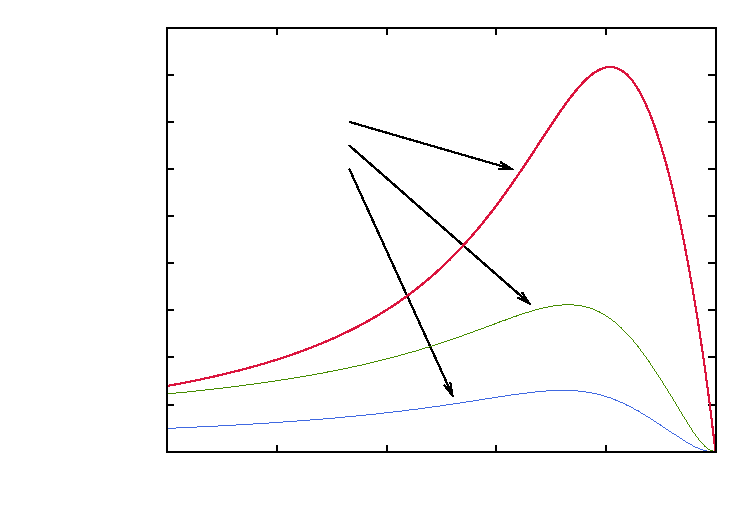
\includegraphics[scale=0.83]{fig_p}}%
    \gplfronttext
  \end{picture}%
\endgroup

        \label{fig:p}
    \end{figure}
\end{frame}



%-------------------------------------------------------------------------------
%---   слайд 11: Решение типовой задачи - решение без шума, динамика состояний
%-------------------------------------------------------------------------------
\begin{frame}
	\frametitle{Решение типовой задачи}
	\framesubtitle{Решение задачи без зашумленности. Динамика состояний $\mathbf{x}(t)$.}
    
    \begin{figure}\center
        % GNUPLOT: LaTeX picture with Postscript
\begingroup
  \makeatletter
  \providecommand\color[2][]{%
    \GenericError{(gnuplot) \space\space\space\@spaces}{%
      Package color not loaded in conjunction with
      terminal option `colourtext'%
    }{See the gnuplot documentation for explanation.%
    }{Either use 'blacktext' in gnuplot or load the package
      color.sty in LaTeX.}%
    \renewcommand\color[2][]{}%
  }%
  \providecommand\includegraphics[2][]{%
    \GenericError{(gnuplot) \space\space\space\@spaces}{%
      Package graphicx or graphics not loaded%
    }{See the gnuplot documentation for explanation.%
    }{The gnuplot epslatex terminal needs graphicx.sty or graphics.sty.}%
    \renewcommand\includegraphics[2][]{}%
  }%
  \providecommand\rotatebox[2]{#2}%
  \@ifundefined{ifGPcolor}{%
    \newif\ifGPcolor
    \GPcolortrue
  }{}%
  \@ifundefined{ifGPblacktext}{%
    \newif\ifGPblacktext
    \GPblacktexttrue
  }{}%
  % define a \g@addto@macro without @ in the name:
  \let\gplgaddtomacro\g@addto@macro
  % define empty templates for all commands taking text:
  \gdef\gplbacktext{}%
  \gdef\gplfronttext{}%
  \makeatother
  \ifGPblacktext
    % no textcolor at all
    \def\colorrgb#1{}%
    \def\colorgray#1{}%
  \else
    % gray or color?
    \ifGPcolor
      \def\colorrgb#1{\color[rgb]{#1}}%
      \def\colorgray#1{\color[gray]{#1}}%
      \expandafter\def\csname LTw\endcsname{\color{white}}%
      \expandafter\def\csname LTb\endcsname{\color{black}}%
      \expandafter\def\csname LTa\endcsname{\color{black}}%
      \expandafter\def\csname LT0\endcsname{\color[rgb]{1,0,0}}%
      \expandafter\def\csname LT1\endcsname{\color[rgb]{0,1,0}}%
      \expandafter\def\csname LT2\endcsname{\color[rgb]{0,0,1}}%
      \expandafter\def\csname LT3\endcsname{\color[rgb]{1,0,1}}%
      \expandafter\def\csname LT4\endcsname{\color[rgb]{0,1,1}}%
      \expandafter\def\csname LT5\endcsname{\color[rgb]{1,1,0}}%
      \expandafter\def\csname LT6\endcsname{\color[rgb]{0,0,0}}%
      \expandafter\def\csname LT7\endcsname{\color[rgb]{1,0.3,0}}%
      \expandafter\def\csname LT8\endcsname{\color[rgb]{0.5,0.5,0.5}}%
    \else
      % gray
      \def\colorrgb#1{\color{black}}%
      \def\colorgray#1{\color[gray]{#1}}%
      \expandafter\def\csname LTw\endcsname{\color{white}}%
      \expandafter\def\csname LTb\endcsname{\color{black}}%
      \expandafter\def\csname LTa\endcsname{\color{black}}%
      \expandafter\def\csname LT0\endcsname{\color{black}}%
      \expandafter\def\csname LT1\endcsname{\color{black}}%
      \expandafter\def\csname LT2\endcsname{\color{black}}%
      \expandafter\def\csname LT3\endcsname{\color{black}}%
      \expandafter\def\csname LT4\endcsname{\color{black}}%
      \expandafter\def\csname LT5\endcsname{\color{black}}%
      \expandafter\def\csname LT6\endcsname{\color{black}}%
      \expandafter\def\csname LT7\endcsname{\color{black}}%
      \expandafter\def\csname LT8\endcsname{\color{black}}%
    \fi
  \fi
  \setlength{\unitlength}{0.0411bp}%
  \begin{picture}(7200.00,5040.00)%
    \gplgaddtomacro\gplbacktext{%
      \csname LTb\endcsname%
      \put(1210,704){\makebox(0,0)[r]{\strut{}-200}}%
      \put(1210,1213){\makebox(0,0)[r]{\strut{} 0}}%
      \put(1210,1722){\makebox(0,0)[r]{\strut{} 200}}%
      \put(1210,2231){\makebox(0,0)[r]{\strut{} 400}}%
      \put(1210,2740){\makebox(0,0)[r]{\strut{} 600}}%
      \put(1210,3248){\makebox(0,0)[r]{\strut{} 800}}%
      \put(1210,3757){\makebox(0,0)[r]{\strut{} 1000}}%
      \put(1210,4266){\makebox(0,0)[r]{\strut{} 1200}}%
      \put(1210,4775){\makebox(0,0)[r]{\strut{} 1400}}%
      \put(1342,484){\makebox(0,0){\strut{} 0}}%
      \put(2447,484){\makebox(0,0){\strut{} 50}}%
      \put(3553,484){\makebox(0,0){\strut{} 100}}%
      \put(4658,484){\makebox(0,0){\strut{} 150}}%
      \put(5764,484){\makebox(0,0){\strut{} 200}}%
      \put(6869,484){\makebox(0,0){\strut{} 250}}%
      \put(308,2739){\rotatebox{-270}{\makebox(0,0){\strut{}Функции состояния}}}%
      \put(4105,154){\makebox(0,0){\strut{}Время, сек}}%
      \put(4282,2994){\makebox(0,0)[l]{\strut{}$x_1(t) \times 10^{-3}$}}%
      \put(2801,1811){\makebox(0,0)[l]{\strut{}$x_2(t) \times 10^{-1}$}}%
      \put(5122,1824){\makebox(0,0)[l]{\strut{}$x_3(t) \times 10^2$}}%
    }%
    \gplgaddtomacro\gplfronttext{%
    }%
    \gplbacktext
    \put(0,0){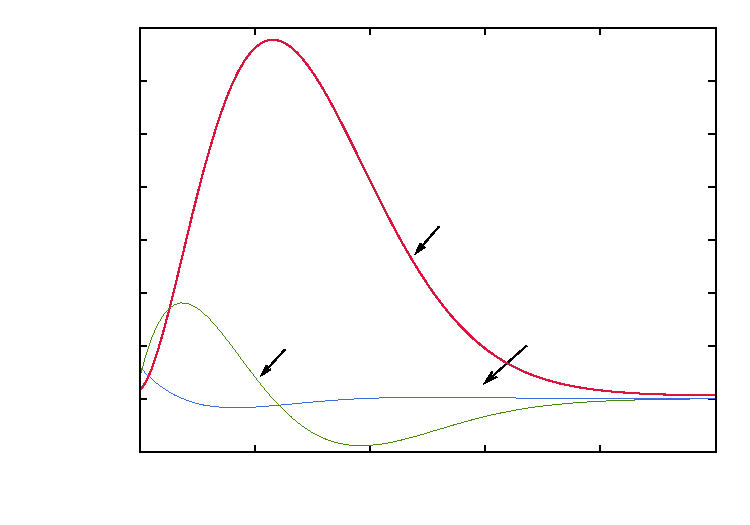
\includegraphics[scale=0.83]{fig_x}}%
    \gplfronttext
  \end{picture}%
\endgroup

        \label{fig:x}
    \end{figure}
\end{frame}



%-------------------------------------------------------------------------------
%---   слайд 12: Решение типовой задачи - алгоритм 1, описание
%-------------------------------------------------------------------------------
\begin{frame}
	\frametitle{Решение типовой задачи}
	\framesubtitle{Описание алгоритма~\ref{alg:1}}
    
    \begin{alg}\label{alg:1}~
        \begin{enumerate}
            \item
                Для заданных $T$, $r$, $\mathbf{Q}(t)$ требуется решить матричное дифференциальное уравнение~\ref{eq:15} в обратном времени с граничным условием $\mathbf{P}(T) = \mathbf{0}$. Таким образом, получим траекторию $\mathbf{P}(t)$, где $0 \leqslant t \leqslant T$;

            \item
                Пользуясь формулой~\ref{eq:14} получаем оптимальное управление $\mathbf{u}^*(t)$ на интервале $0 \leqslant t \leqslant T$ в каждый момент времени $t$.
        \end{enumerate}
    \end{alg}
\end{frame}



%-------------------------------------------------------------------------------
%---   слайд 13: Решение типовой задачи - алгоритм 1, результаты
%-------------------------------------------------------------------------------
\begin{frame}
	\frametitle{Решение типовой задачи}
	\framesubtitle{Решение задачи с помощью алгоритма~\ref{alg:1}}
    
    \begin{figure}\center
        % GNUPLOT: LaTeX picture with Postscript
\begingroup
  \makeatletter
  \providecommand\color[2][]{%
    \GenericError{(gnuplot) \space\space\space\@spaces}{%
      Package color not loaded in conjunction with
      terminal option `colourtext'%
    }{See the gnuplot documentation for explanation.%
    }{Either use 'blacktext' in gnuplot or load the package
      color.sty in LaTeX.}%
    \renewcommand\color[2][]{}%
  }%
  \providecommand\includegraphics[2][]{%
    \GenericError{(gnuplot) \space\space\space\@spaces}{%
      Package graphicx or graphics not loaded%
    }{See the gnuplot documentation for explanation.%
    }{The gnuplot epslatex terminal needs graphicx.sty or graphics.sty.}%
    \renewcommand\includegraphics[2][]{}%
  }%
  \providecommand\rotatebox[2]{#2}%
  \@ifundefined{ifGPcolor}{%
    \newif\ifGPcolor
    \GPcolortrue
  }{}%
  \@ifundefined{ifGPblacktext}{%
    \newif\ifGPblacktext
    \GPblacktexttrue
  }{}%
  % define a \g@addto@macro without @ in the name:
  \let\gplgaddtomacro\g@addto@macro
  % define empty templates for all commands taking text:
  \gdef\gplbacktext{}%
  \gdef\gplfronttext{}%
  \makeatother
  \ifGPblacktext
    % no textcolor at all
    \def\colorrgb#1{}%
    \def\colorgray#1{}%
  \else
    % gray or color?
    \ifGPcolor
      \def\colorrgb#1{\color[rgb]{#1}}%
      \def\colorgray#1{\color[gray]{#1}}%
      \expandafter\def\csname LTw\endcsname{\color{white}}%
      \expandafter\def\csname LTb\endcsname{\color{black}}%
      \expandafter\def\csname LTa\endcsname{\color{black}}%
      \expandafter\def\csname LT0\endcsname{\color[rgb]{1,0,0}}%
      \expandafter\def\csname LT1\endcsname{\color[rgb]{0,1,0}}%
      \expandafter\def\csname LT2\endcsname{\color[rgb]{0,0,1}}%
      \expandafter\def\csname LT3\endcsname{\color[rgb]{1,0,1}}%
      \expandafter\def\csname LT4\endcsname{\color[rgb]{0,1,1}}%
      \expandafter\def\csname LT5\endcsname{\color[rgb]{1,1,0}}%
      \expandafter\def\csname LT6\endcsname{\color[rgb]{0,0,0}}%
      \expandafter\def\csname LT7\endcsname{\color[rgb]{1,0.3,0}}%
      \expandafter\def\csname LT8\endcsname{\color[rgb]{0.5,0.5,0.5}}%
    \else
      % gray
      \def\colorrgb#1{\color{black}}%
      \def\colorgray#1{\color[gray]{#1}}%
      \expandafter\def\csname LTw\endcsname{\color{white}}%
      \expandafter\def\csname LTb\endcsname{\color{black}}%
      \expandafter\def\csname LTa\endcsname{\color{black}}%
      \expandafter\def\csname LT0\endcsname{\color{black}}%
      \expandafter\def\csname LT1\endcsname{\color{black}}%
      \expandafter\def\csname LT2\endcsname{\color{black}}%
      \expandafter\def\csname LT3\endcsname{\color{black}}%
      \expandafter\def\csname LT4\endcsname{\color{black}}%
      \expandafter\def\csname LT5\endcsname{\color{black}}%
      \expandafter\def\csname LT6\endcsname{\color{black}}%
      \expandafter\def\csname LT7\endcsname{\color{black}}%
      \expandafter\def\csname LT8\endcsname{\color{black}}%
    \fi
  \fi
  \setlength{\unitlength}{0.0411bp}%
  \begin{picture}(7200.00,5040.00)%
    \gplgaddtomacro\gplbacktext{%
      \csname LTb\endcsname%
      \put(1210,704){\makebox(0,0)[r]{\strut{}-400}}%
      \put(1210,1156){\makebox(0,0)[r]{\strut{}-200}}%
      \put(1210,1609){\makebox(0,0)[r]{\strut{} 0}}%
      \put(1210,2061){\makebox(0,0)[r]{\strut{} 200}}%
      \put(1210,2513){\makebox(0,0)[r]{\strut{} 400}}%
      \put(1210,2966){\makebox(0,0)[r]{\strut{} 600}}%
      \put(1210,3418){\makebox(0,0)[r]{\strut{} 800}}%
      \put(1210,3870){\makebox(0,0)[r]{\strut{} 1000}}%
      \put(1210,4323){\makebox(0,0)[r]{\strut{} 1200}}%
      \put(1210,4775){\makebox(0,0)[r]{\strut{} 1400}}%
      \put(1342,484){\makebox(0,0){\strut{} 0}}%
      \put(2447,484){\makebox(0,0){\strut{} 50}}%
      \put(3553,484){\makebox(0,0){\strut{} 100}}%
      \put(4658,484){\makebox(0,0){\strut{} 150}}%
      \put(5764,484){\makebox(0,0){\strut{} 200}}%
      \put(6869,484){\makebox(0,0){\strut{} 250}}%
      \put(308,2739){\rotatebox{-270}{\makebox(0,0){\strut{}Функции состояния}}}%
      \put(4105,154){\makebox(0,0){\strut{}Время, сек}}%
      \put(4017,3192){\makebox(0,0)[l]{\strut{}$x_1(t) \times 10^{-3}$}}%
      \put(2293,2807){\makebox(0,0)[l]{\strut{}$x_2(t) \times 10^{-1}$}}%
      \put(5122,2151){\makebox(0,0)[l]{\strut{}$x_3(t) \times 10^2$}}%
    }%
    \gplgaddtomacro\gplfronttext{%
    }%
    \gplbacktext
    \put(0,0){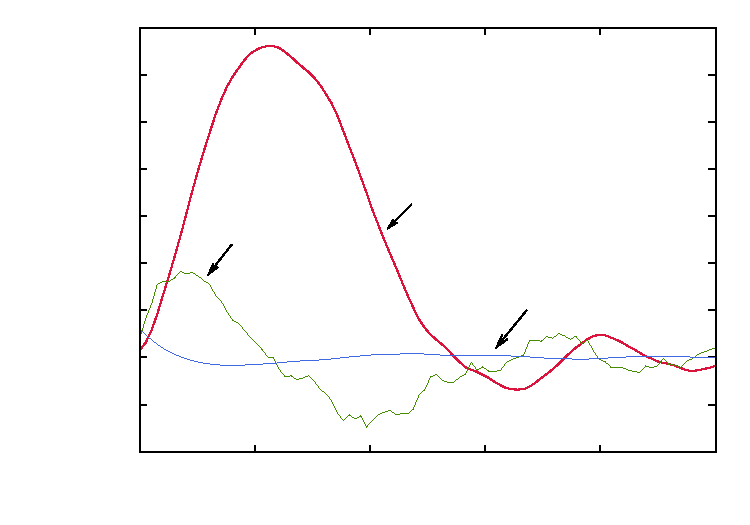
\includegraphics[scale=0.84]{fig_alg1}}%
    \gplfronttext
  \end{picture}%
\endgroup

        \label{fig:alg1}
    \end{figure}
\end{frame}



%-------------------------------------------------------------------------------
%---   слайд 15: Решение типовой задачи - алгоритм 2, описание
%-------------------------------------------------------------------------------
\begin{frame}
	\frametitle{Решение типовой задачи}
	\framesubtitle{Описание алгоритма~\ref{alg:2}}
    
    \begin{alg}\label{alg:2}~
        \begin{enumerate}
            \item
                Для заданных $T$, $r$, $\mathbf{Q}(t)$ требуется решить матричное алгербаическое уравнение~\ref{eq:10}. Таким образом, получим матрицу усилений $\mathbf{P}$ для всех $t$ из $0 \leqslant t \leqslant T$;

            \item
                Пользуясь формулой~\ref{eq:9} получаем оптимальное управление $\mathbf{u}^*(t)$ на интервале $0 \leqslant t \leqslant T$ в каждый момент времени $t$.
        \end{enumerate}
    \end{alg}
\end{frame}



%-------------------------------------------------------------------------------
%---   слайд 15: Решение типовой задачи - алгоритм 2, результаты
%-------------------------------------------------------------------------------
\begin{frame}
	\frametitle{Решение типовой задачи}
	\framesubtitle{Решение задачи с помощью алгоритма~\ref{alg:2}}
    
    \begin{figure}\center
        % GNUPLOT: LaTeX picture with Postscript
\begingroup
  \makeatletter
  \providecommand\color[2][]{%
    \GenericError{(gnuplot) \space\space\space\@spaces}{%
      Package color not loaded in conjunction with
      terminal option `colourtext'%
    }{See the gnuplot documentation for explanation.%
    }{Either use 'blacktext' in gnuplot or load the package
      color.sty in LaTeX.}%
    \renewcommand\color[2][]{}%
  }%
  \providecommand\includegraphics[2][]{%
    \GenericError{(gnuplot) \space\space\space\@spaces}{%
      Package graphicx or graphics not loaded%
    }{See the gnuplot documentation for explanation.%
    }{The gnuplot epslatex terminal needs graphicx.sty or graphics.sty.}%
    \renewcommand\includegraphics[2][]{}%
  }%
  \providecommand\rotatebox[2]{#2}%
  \@ifundefined{ifGPcolor}{%
    \newif\ifGPcolor
    \GPcolortrue
  }{}%
  \@ifundefined{ifGPblacktext}{%
    \newif\ifGPblacktext
    \GPblacktexttrue
  }{}%
  % define a \g@addto@macro without @ in the name:
  \let\gplgaddtomacro\g@addto@macro
  % define empty templates for all commands taking text:
  \gdef\gplbacktext{}%
  \gdef\gplfronttext{}%
  \makeatother
  \ifGPblacktext
    % no textcolor at all
    \def\colorrgb#1{}%
    \def\colorgray#1{}%
  \else
    % gray or color?
    \ifGPcolor
      \def\colorrgb#1{\color[rgb]{#1}}%
      \def\colorgray#1{\color[gray]{#1}}%
      \expandafter\def\csname LTw\endcsname{\color{white}}%
      \expandafter\def\csname LTb\endcsname{\color{black}}%
      \expandafter\def\csname LTa\endcsname{\color{black}}%
      \expandafter\def\csname LT0\endcsname{\color[rgb]{1,0,0}}%
      \expandafter\def\csname LT1\endcsname{\color[rgb]{0,1,0}}%
      \expandafter\def\csname LT2\endcsname{\color[rgb]{0,0,1}}%
      \expandafter\def\csname LT3\endcsname{\color[rgb]{1,0,1}}%
      \expandafter\def\csname LT4\endcsname{\color[rgb]{0,1,1}}%
      \expandafter\def\csname LT5\endcsname{\color[rgb]{1,1,0}}%
      \expandafter\def\csname LT6\endcsname{\color[rgb]{0,0,0}}%
      \expandafter\def\csname LT7\endcsname{\color[rgb]{1,0.3,0}}%
      \expandafter\def\csname LT8\endcsname{\color[rgb]{0.5,0.5,0.5}}%
    \else
      % gray
      \def\colorrgb#1{\color{black}}%
      \def\colorgray#1{\color[gray]{#1}}%
      \expandafter\def\csname LTw\endcsname{\color{white}}%
      \expandafter\def\csname LTb\endcsname{\color{black}}%
      \expandafter\def\csname LTa\endcsname{\color{black}}%
      \expandafter\def\csname LT0\endcsname{\color{black}}%
      \expandafter\def\csname LT1\endcsname{\color{black}}%
      \expandafter\def\csname LT2\endcsname{\color{black}}%
      \expandafter\def\csname LT3\endcsname{\color{black}}%
      \expandafter\def\csname LT4\endcsname{\color{black}}%
      \expandafter\def\csname LT5\endcsname{\color{black}}%
      \expandafter\def\csname LT6\endcsname{\color{black}}%
      \expandafter\def\csname LT7\endcsname{\color{black}}%
      \expandafter\def\csname LT8\endcsname{\color{black}}%
    \fi
  \fi
  \setlength{\unitlength}{0.0411bp}%
  \begin{picture}(7200.00,5040.00)%
    \gplgaddtomacro\gplbacktext{%
      \csname LTb\endcsname%
      \put(1342,704){\makebox(0,0)[r]{\strut{}-15000}}%
      \put(1342,1383){\makebox(0,0)[r]{\strut{}-10000}}%
      \put(1342,2061){\makebox(0,0)[r]{\strut{}-5000}}%
      \put(1342,2740){\makebox(0,0)[r]{\strut{} 0}}%
      \put(1342,3418){\makebox(0,0)[r]{\strut{} 5000}}%
      \put(1342,4097){\makebox(0,0)[r]{\strut{} 10000}}%
      \put(1342,4775){\makebox(0,0)[r]{\strut{} 15000}}%
      \put(1474,484){\makebox(0,0){\strut{} 0}}%
      \put(2553,484){\makebox(0,0){\strut{} 50}}%
      \put(3632,484){\makebox(0,0){\strut{} 100}}%
      \put(4711,484){\makebox(0,0){\strut{} 150}}%
      \put(5790,484){\makebox(0,0){\strut{} 200}}%
      \put(6869,484){\makebox(0,0){\strut{} 250}}%
      \put(308,2739){\rotatebox{-270}{\makebox(0,0){\strut{}Функции состояния}}}%
      \put(4171,154){\makebox(0,0){\strut{}Время, сек}}%
      \put(5143,4273){\makebox(0,0){\strut{}$x_1(t) \times 10^{-3}$}}%
      \put(5574,1111){\makebox(0,0){\strut{}$x_2(t) \times 10^{-1}$}}%
      \put(2834,3974){\makebox(0,0)[r]{\strut{}$x_3(t) \times 10^2$}}%
    }%
    \gplgaddtomacro\gplfronttext{%
    }%
    \gplbacktext
    \put(0,0){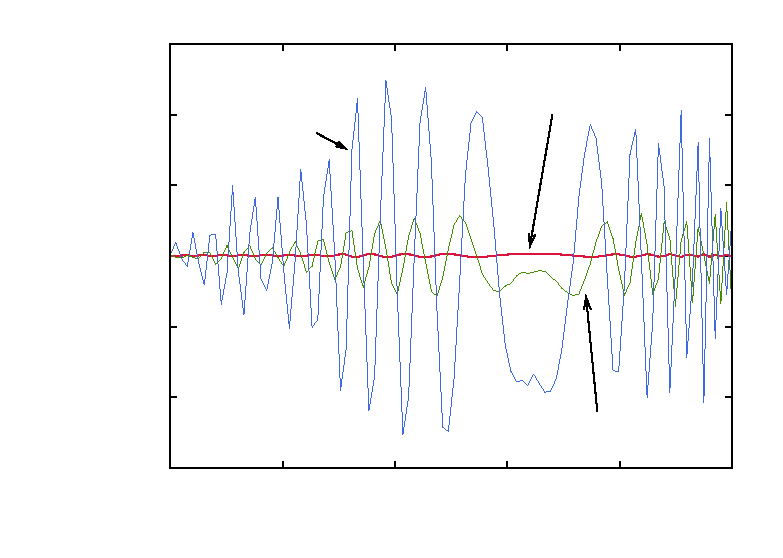
\includegraphics[scale=0.83]{fig_alg2}}%
    \gplfronttext
  \end{picture}%
\endgroup

        \label{fig:alg2}
    \end{figure}
\end{frame}



%-------------------------------------------------------------------------------
%---   слайд 16: Решение типовой задачи - вторичный критерий качества
%-------------------------------------------------------------------------------
\begin{frame}
	\frametitle{Решение типовой задачи}
	\framesubtitle{Вторичный критерий качества}
    
    \begin{equation}\label{eq:18}
        \begin{split}
            \mathscr{S}(\mathbf{x}, t_i, t_{i+1}) =&~ \Biggl| \int\limits_{t_i}^{t_{i+1}} \bigl( \mathbf{x}^T(\tau)\mathbf{Q}(\tau)\mathbf{x}(\tau) + ru(\tau)^2 \bigr)\,d\tau -\\
            &- 2\mathcal{F}^*(\mathbf{x}, t_i, t_{i+1}) \Biggr| \text{.}
        \end{split}
    \end{equation}
\end{frame}



%-------------------------------------------------------------------------------
%---   слайд 17: Решение типовой задачи - алгоритм 3, описание
%-------------------------------------------------------------------------------
\begin{frame}
	\frametitle{Решение типовой задачи}
	\framesubtitle{Описание алгоритма~\ref{alg:3}}\small
    
    \begin{alg}\label{alg:3}~
        \begin{enumerate}
            \item
                Делим временной интервал наблюдений $[0, T]$ на $n+1$ равную часть: $0 = t_0 < t_1 < t_2 < \ldots < t_{n} = T$, где $t_{i+1}-t_i = t_{j+1}-t_j$ для всех $i, j < n$. Интервалы типа $[t_i, t_{i+1})$ ($i<n$) назовем \emph{подынтервалами};

            \item
                Строим оптимальное управление $\mathbf{u}^*$ на всем оставшемся интервале наблюдений с помощью алгоритмов~\ref{alg:1} или~\ref{alg:2};

            \item
                Наводим ракету с помощью управления $\mathbf{u}^*$ на протяжении одного подынтервала времени;

            \item
                На открытой границе подынтервала производим расчет вторичного критерия $\mathscr{S}(\mathbf{x}, t_i, t_{i+1})$ (например, заданного уравнением~\ref{eq:18});

            \item
                Если $\mathscr{S}(\mathbf{x}, t_i, t_{i+1}) \leqslant \varepsilon$ ($\varepsilon > 0$), то переходим на шаг 3, в противном случае переходим на шаг 2.
        \end{enumerate}
    \end{alg}
\end{frame}



%-------------------------------------------------------------------------------
%---   слайд 18: Решение типовой задачи - алгоритм 3, результаты
%-------------------------------------------------------------------------------
\begin{frame}
	\frametitle{Решение типовой задачи}
	\framesubtitle{Решение задачи с помощью алгоритма~\ref{alg:3}}
    
    \begin{figure}\center
        % GNUPLOT: LaTeX picture with Postscript
\begingroup
  \makeatletter
  \providecommand\color[2][]{%
    \GenericError{(gnuplot) \space\space\space\@spaces}{%
      Package color not loaded in conjunction with
      terminal option `colourtext'%
    }{See the gnuplot documentation for explanation.%
    }{Either use 'blacktext' in gnuplot or load the package
      color.sty in LaTeX.}%
    \renewcommand\color[2][]{}%
  }%
  \providecommand\includegraphics[2][]{%
    \GenericError{(gnuplot) \space\space\space\@spaces}{%
      Package graphicx or graphics not loaded%
    }{See the gnuplot documentation for explanation.%
    }{The gnuplot epslatex terminal needs graphicx.sty or graphics.sty.}%
    \renewcommand\includegraphics[2][]{}%
  }%
  \providecommand\rotatebox[2]{#2}%
  \@ifundefined{ifGPcolor}{%
    \newif\ifGPcolor
    \GPcolortrue
  }{}%
  \@ifundefined{ifGPblacktext}{%
    \newif\ifGPblacktext
    \GPblacktexttrue
  }{}%
  % define a \g@addto@macro without @ in the name:
  \let\gplgaddtomacro\g@addto@macro
  % define empty templates for all commands taking text:
  \gdef\gplbacktext{}%
  \gdef\gplfronttext{}%
  \makeatother
  \ifGPblacktext
    % no textcolor at all
    \def\colorrgb#1{}%
    \def\colorgray#1{}%
  \else
    % gray or color?
    \ifGPcolor
      \def\colorrgb#1{\color[rgb]{#1}}%
      \def\colorgray#1{\color[gray]{#1}}%
      \expandafter\def\csname LTw\endcsname{\color{white}}%
      \expandafter\def\csname LTb\endcsname{\color{black}}%
      \expandafter\def\csname LTa\endcsname{\color{black}}%
      \expandafter\def\csname LT0\endcsname{\color[rgb]{1,0,0}}%
      \expandafter\def\csname LT1\endcsname{\color[rgb]{0,1,0}}%
      \expandafter\def\csname LT2\endcsname{\color[rgb]{0,0,1}}%
      \expandafter\def\csname LT3\endcsname{\color[rgb]{1,0,1}}%
      \expandafter\def\csname LT4\endcsname{\color[rgb]{0,1,1}}%
      \expandafter\def\csname LT5\endcsname{\color[rgb]{1,1,0}}%
      \expandafter\def\csname LT6\endcsname{\color[rgb]{0,0,0}}%
      \expandafter\def\csname LT7\endcsname{\color[rgb]{1,0.3,0}}%
      \expandafter\def\csname LT8\endcsname{\color[rgb]{0.5,0.5,0.5}}%
    \else
      % gray
      \def\colorrgb#1{\color{black}}%
      \def\colorgray#1{\color[gray]{#1}}%
      \expandafter\def\csname LTw\endcsname{\color{white}}%
      \expandafter\def\csname LTb\endcsname{\color{black}}%
      \expandafter\def\csname LTa\endcsname{\color{black}}%
      \expandafter\def\csname LT0\endcsname{\color{black}}%
      \expandafter\def\csname LT1\endcsname{\color{black}}%
      \expandafter\def\csname LT2\endcsname{\color{black}}%
      \expandafter\def\csname LT3\endcsname{\color{black}}%
      \expandafter\def\csname LT4\endcsname{\color{black}}%
      \expandafter\def\csname LT5\endcsname{\color{black}}%
      \expandafter\def\csname LT6\endcsname{\color{black}}%
      \expandafter\def\csname LT7\endcsname{\color{black}}%
      \expandafter\def\csname LT8\endcsname{\color{black}}%
    \fi
  \fi
  \setlength{\unitlength}{0.0411bp}%
  \begin{picture}(7200.00,5040.00)%
    \gplgaddtomacro\gplbacktext{%
      \csname LTb\endcsname%
      \put(1210,704){\makebox(0,0)[r]{\strut{}-400}}%
      \put(1210,1111){\makebox(0,0)[r]{\strut{}-200}}%
      \put(1210,1518){\makebox(0,0)[r]{\strut{} 0}}%
      \put(1210,1925){\makebox(0,0)[r]{\strut{} 200}}%
      \put(1210,2332){\makebox(0,0)[r]{\strut{} 400}}%
      \put(1210,2740){\makebox(0,0)[r]{\strut{} 600}}%
      \put(1210,3147){\makebox(0,0)[r]{\strut{} 800}}%
      \put(1210,3554){\makebox(0,0)[r]{\strut{} 1000}}%
      \put(1210,3961){\makebox(0,0)[r]{\strut{} 1200}}%
      \put(1210,4368){\makebox(0,0)[r]{\strut{} 1400}}%
      \put(1210,4775){\makebox(0,0)[r]{\strut{} 1600}}%
      \put(1342,484){\makebox(0,0){\strut{} 0}}%
      \put(2447,484){\makebox(0,0){\strut{} 50}}%
      \put(3553,484){\makebox(0,0){\strut{} 100}}%
      \put(4658,484){\makebox(0,0){\strut{} 150}}%
      \put(5764,484){\makebox(0,0){\strut{} 200}}%
      \put(6869,484){\makebox(0,0){\strut{} 250}}%
      \put(308,2739){\rotatebox{-270}{\makebox(0,0){\strut{}Функции состояния}}}%
      \put(4105,154){\makebox(0,0){\strut{}Время, сек}}%
      \put(4481,3187){\makebox(0,0)[l]{\strut{}$x_1(t) \times 10^{-3}$}}%
      \put(2646,2373){\makebox(0,0)[l]{\strut{}$x_2(t) \times 10^{-1}$}}%
      \put(4481,1050){\makebox(0,0)[l]{\strut{}$x_3(t) \times 10^2$}}%
    }%
    \gplgaddtomacro\gplfronttext{%
    }%
    \gplbacktext
    \put(0,0){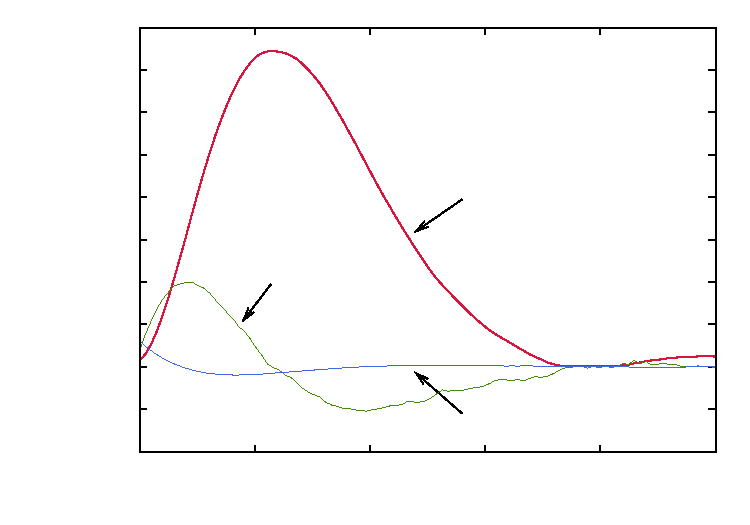
\includegraphics[scale=0.83]{fig_alg3}}%
    \gplfronttext
  \end{picture}%
\endgroup

        \label{fig:alg3}
    \end{figure}
\end{frame}



%-------------------------------------------------------------------------------
%---   слайд 19: Решение типовой задачи - алгоритм 4, описание
%-------------------------------------------------------------------------------
\begin{frame}
	\frametitle{Решение типовой задачи}
	\framesubtitle{Описание алгоритма~\ref{alg:4}}\footnotesize
    
    \begin{alg}\label{alg:4}~
        \begin{enumerate}
            \item
                Делим временной интервал наблюдений $[0, T]$ на $n+1$ равную часть: $0 = t_0 < t_1 < t_2 < \ldots < t_{n} = T$, где $t_{i+1}-t_i = t_{j+1}-t_j$ для всех $i, j < n$. Интервалы типа $[t_i, t_{i+1})$ ($i<n$) назовем подынтервалами. Оптимальное управление строится поподынтервально;

            \item
                Строим оптимальное управление $\mathbf{u}^*$ только лишь на следующем подынтервале с помощью алгоритмов~\ref{alg:1} или~\ref{alg:2};

            \item
                Наводим ракету с помощью управления $\mathbf{u}^*$ на протяжении одного подынтервала времени;

            \item
                На открытой границе подынтервала производим расчет вторичного критерия $\mathscr{S}(\mathbf{x}, t_i, t_{i+1})$ (например, заданного уравнением~\ref{eq:18});

            \item
                Если $\mathscr{S}(\mathbf{x}, t_i, t_{i+1}) > \varepsilon$ ($\varepsilon > 0$), то сразу переходим на шаг 2. В противном случае, также переходим на шаг 2, но в качестве следующего подынтервала рассматриваем интервал удвоенной длины, если оставшихся подынтервалов достаточно (если нет~--- берется оставшийся временной промежуток).
        \end{enumerate}
    \end{alg}
\end{frame}



%-------------------------------------------------------------------------------
%---   слайд 20: Решение типовой задачи - алгоритм 4, результаты
%-------------------------------------------------------------------------------
\begin{frame}
	\frametitle{Решение типовой задачи}
	\framesubtitle{Решение задачи с помощью алгоритма~\ref{alg:4}}
    
    \begin{figure}\center
        % GNUPLOT: LaTeX picture with Postscript
\begingroup
  \makeatletter
  \providecommand\color[2][]{%
    \GenericError{(gnuplot) \space\space\space\@spaces}{%
      Package color not loaded in conjunction with
      terminal option `colourtext'%
    }{See the gnuplot documentation for explanation.%
    }{Either use 'blacktext' in gnuplot or load the package
      color.sty in LaTeX.}%
    \renewcommand\color[2][]{}%
  }%
  \providecommand\includegraphics[2][]{%
    \GenericError{(gnuplot) \space\space\space\@spaces}{%
      Package graphicx or graphics not loaded%
    }{See the gnuplot documentation for explanation.%
    }{The gnuplot epslatex terminal needs graphicx.sty or graphics.sty.}%
    \renewcommand\includegraphics[2][]{}%
  }%
  \providecommand\rotatebox[2]{#2}%
  \@ifundefined{ifGPcolor}{%
    \newif\ifGPcolor
    \GPcolortrue
  }{}%
  \@ifundefined{ifGPblacktext}{%
    \newif\ifGPblacktext
    \GPblacktexttrue
  }{}%
  % define a \g@addto@macro without @ in the name:
  \let\gplgaddtomacro\g@addto@macro
  % define empty templates for all commands taking text:
  \gdef\gplbacktext{}%
  \gdef\gplfronttext{}%
  \makeatother
  \ifGPblacktext
    % no textcolor at all
    \def\colorrgb#1{}%
    \def\colorgray#1{}%
  \else
    % gray or color?
    \ifGPcolor
      \def\colorrgb#1{\color[rgb]{#1}}%
      \def\colorgray#1{\color[gray]{#1}}%
      \expandafter\def\csname LTw\endcsname{\color{white}}%
      \expandafter\def\csname LTb\endcsname{\color{black}}%
      \expandafter\def\csname LTa\endcsname{\color{black}}%
      \expandafter\def\csname LT0\endcsname{\color[rgb]{1,0,0}}%
      \expandafter\def\csname LT1\endcsname{\color[rgb]{0,1,0}}%
      \expandafter\def\csname LT2\endcsname{\color[rgb]{0,0,1}}%
      \expandafter\def\csname LT3\endcsname{\color[rgb]{1,0,1}}%
      \expandafter\def\csname LT4\endcsname{\color[rgb]{0,1,1}}%
      \expandafter\def\csname LT5\endcsname{\color[rgb]{1,1,0}}%
      \expandafter\def\csname LT6\endcsname{\color[rgb]{0,0,0}}%
      \expandafter\def\csname LT7\endcsname{\color[rgb]{1,0.3,0}}%
      \expandafter\def\csname LT8\endcsname{\color[rgb]{0.5,0.5,0.5}}%
    \else
      % gray
      \def\colorrgb#1{\color{black}}%
      \def\colorgray#1{\color[gray]{#1}}%
      \expandafter\def\csname LTw\endcsname{\color{white}}%
      \expandafter\def\csname LTb\endcsname{\color{black}}%
      \expandafter\def\csname LTa\endcsname{\color{black}}%
      \expandafter\def\csname LT0\endcsname{\color{black}}%
      \expandafter\def\csname LT1\endcsname{\color{black}}%
      \expandafter\def\csname LT2\endcsname{\color{black}}%
      \expandafter\def\csname LT3\endcsname{\color{black}}%
      \expandafter\def\csname LT4\endcsname{\color{black}}%
      \expandafter\def\csname LT5\endcsname{\color{black}}%
      \expandafter\def\csname LT6\endcsname{\color{black}}%
      \expandafter\def\csname LT7\endcsname{\color{black}}%
      \expandafter\def\csname LT8\endcsname{\color{black}}%
    \fi
  \fi
  \setlength{\unitlength}{0.0411bp}%
  \begin{picture}(7200.00,5040.00)%
    \gplgaddtomacro\gplbacktext{%
      \csname LTb\endcsname%
      \put(1474,704){\makebox(0,0)[r]{\strut{}-20000}}%
      \put(1474,1213){\makebox(0,0)[r]{\strut{} 0}}%
      \put(1474,1722){\makebox(0,0)[r]{\strut{} 20000}}%
      \put(1474,2231){\makebox(0,0)[r]{\strut{} 40000}}%
      \put(1474,2740){\makebox(0,0)[r]{\strut{} 60000}}%
      \put(1474,3248){\makebox(0,0)[r]{\strut{} 80000}}%
      \put(1474,3757){\makebox(0,0)[r]{\strut{} 100000}}%
      \put(1474,4266){\makebox(0,0)[r]{\strut{} 120000}}%
      \put(1474,4775){\makebox(0,0)[r]{\strut{} 140000}}%
      \put(1606,484){\makebox(0,0){\strut{} 0}}%
      \put(2659,484){\makebox(0,0){\strut{} 50}}%
      \put(3711,484){\makebox(0,0){\strut{} 100}}%
      \put(4764,484){\makebox(0,0){\strut{} 150}}%
      \put(5816,484){\makebox(0,0){\strut{} 200}}%
      \put(6869,484){\makebox(0,0){\strut{} 250}}%
      \put(308,2739){\rotatebox{-270}{\makebox(0,0){\strut{}Функции состояния}}}%
      \put(4237,154){\makebox(0,0){\strut{}Время, сек}}%
      \put(3501,3579){\makebox(0,0)[r]{\strut{}$x_1(t) \times 10^{-3}$}}%
      \put(3522,1976){\makebox(0,0)[l]{\strut{}$x_2(t) \times 10^{-1}$}}%
      \put(5185,2638){\makebox(0,0){\strut{}$x_3(t) \times 10^2$}}%
    }%
    \gplgaddtomacro\gplfronttext{%
    }%
    \gplbacktext
    \put(0,0){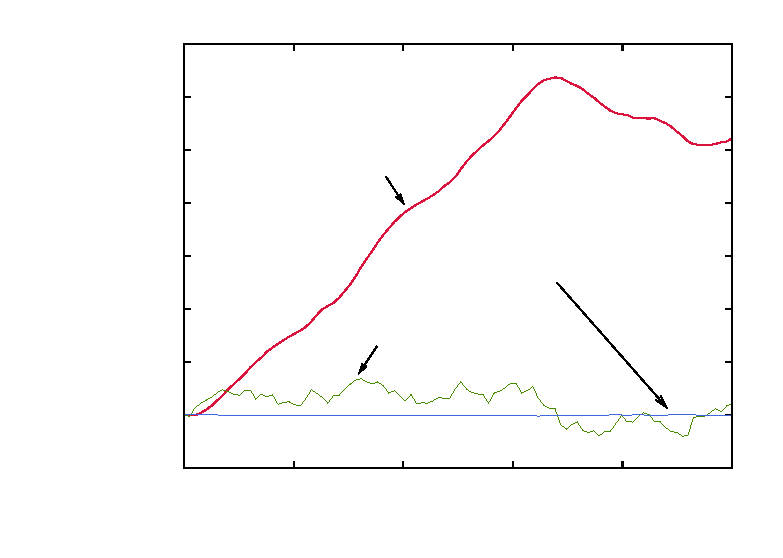
\includegraphics[scale=0.83]{fig_alg4}}%
    \gplfronttext
  \end{picture}%
\endgroup

        \label{fig:alg4}
    \end{figure}
\end{frame}



%-------------------------------------------------------------------------------
%---   слайд 21: Заключение
%-------------------------------------------------------------------------------
\begin{frame}
	\frametitle{Заключение}
    
    \begin{enumerate}
        \item
            Исследована исходная задача управления;

        \item
            Дан общий метод синтеза оптимального управления, основывающийся на уравнениях Беллмана; даны решения задачи в некоторых частных случаях;

        \item
            Полученные результаты распространены на случай стохастических систем;

        \item
            Были разработаны алгоритмы решения задачи синтеза оптимального управления на примере конкретной задачи;

        \item
            Разработан программный комплекс для исследования и анализа алгоритмов;

        \item
            Полученные результаты были проанализированы, даны рекомендации по использованию алгоритмов.
    \end{enumerate}
\end{frame}



\end{document}

